\documentclass[11pt]{article}

\usepackage[margin=1in]{geometry}
\usepackage{amsmath,amssymb,amsfonts}
\usepackage{booktabs}
\usepackage{graphicx}
\usepackage{hyperref}
\usepackage[numbers,sort&compress]{natbib}

\title{Quantum Latent Consistency Models for Few-Step Synthetic Image Generation}
\author{Felipe Mahlow\thanks{Manuscript in preparation. Affiliation and acknowledgements to be completed.}}
\date{\today}

\begin{document}

\maketitle

\begin{abstract}
Diffusion models have become a leading approach to image synthesis, but their
iterative sampling procedures remain expensive. Consistency models and latent
consistency models reduce this cost by learning mappings that send noisy points
along a diffusion trajectory directly toward a common clean endpoint. In
parallel, quantum generative learning has explored parameterized quantum circuits
as compact function classes for near-term quantum machine learning, including
recent quantum denoising diffusion models. This paper proposes Quantum Latent
Consistency Models (QLCMs), a hybrid quantum-classical architecture that
distills a latent diffusion teacher into a parameterized quantum consistency
student. The student receives a noisy latent state and a noise level, encodes
them into a simulated variational quantum circuit, and predicts a clean latent
endpoint or a residual correction to a classical consistency head. We formulate
the QLCM training objective, describe one-step and few-step samplers, and propose
a controlled evaluation protocol on MNIST and Fashion-MNIST against
parameter-matched classical consistency students and latent diffusion baselines.
The central question is not whether the model demonstrates quantum advantage,
but whether quantum consistency modules provide useful inductive bias or
parameter efficiency in low-dimensional latent image generation. In simulator
experiments on MNIST and Fashion-MNIST, the residual quantum placement
(QLCM-R) does not outperform a parameter-matched classical consistency
student: across three seeds it has 54\% more trainable parameters
(139{,}640 vs. 90{,}640) and a slightly worse classifier-feature FID-like
score ($391.7\pm4.7$ vs. $382.9\pm5.5$), with statistically indistinguishable
sample diversity and recognizability. Using the quantum circuit as the
primary consistency head (QLCM-H) trains to a substantially higher loss and
collapses sample diversity (label entropy 1.2--1.7 vs. $\approx$2.0 out of a
maximum of 2.303), confirming a failure mode anticipated at the design stage.
We report this as a negative result for the architectures and dataset scale
tested, together with the full evidence package needed to reproduce or
challenge it.
\end{abstract}

\textbf{Keywords:} quantum machine learning; consistency models; latent
diffusion; generative modeling; synthetic image generation; variational quantum
circuits

\section{Introduction}

Denoising diffusion probabilistic models (DDPMs) generate high-quality images by
learning to reverse a gradual noising process \citep{ho2020ddpm}. Their
performance has made diffusion-based methods a central class of modern
generative models, but sampling typically requires many neural function
evaluations. Latent diffusion models (LDMs) reduce the computational burden by
moving the denoising process from pixel space into the latent space of an
autoencoder \citep{rombach2022ldm}. Consistency models address a different part
of the same bottleneck: instead of learning only a local denoising step, they
learn a map that sends points along a probability-flow trajectory to a common
clean endpoint, allowing one-step or few-step generation
\citep{song2023consistency}. Latent Consistency Models (LCMs) combine this idea
with latent diffusion and demonstrate fast synthesis through consistency
distillation \citep{luo2023lcm}.

Quantum machine learning offers another route for compact generative modeling.
Parameterized quantum circuits can represent nonlinear feature maps and
trainable measurement functions, and quantum generative models have been
studied across adversarial, Born-machine, and diffusion-inspired formulations.
Recent quantum denoising diffusion work has brought diffusion-style training
into quantum and hybrid settings, including image-oriented quantum denoising
architectures, a quantum single-sampling consistency-inspired architecture, and
quantum-data diffusion models
\citep{kolle2024qddm,zhang2023quddpm,kwun2024mixedquddpm}. These results show
that the intersection of quantum circuits and diffusion models is already
active. They also make broad novelty claims inappropriate: a new contribution
must specify what changes in the learning objective, architecture, and empirical
question.

This paper proposes Quantum Latent Consistency Models (QLCMs). QLCMs transfer
the consistency-model objective into a hybrid quantum-classical latent image
generator. A classical encoder maps an image to a compact latent vector. A
classical latent diffusion teacher defines trajectories in this latent space. A
hybrid student then learns a consistency function in which a parameterized
quantum circuit contributes either the direct clean-latent prediction, a
time-conditioning signal, or a residual correction to a classical consistency
head. This design differs from prior quantum image diffusion work by combining
latent-space teacher-student consistency distillation with explicit ablations of
where a quantum circuit should enter the consistency map.

The intended contributions are:
\begin{enumerate}
    \item a formal QLCM architecture for simulator-based few-step image
    generation;
    \item three quantum consistency placements: direct head, residual
    correction, and time-conditioning;
    \item a distillation objective that adapts latent consistency training to a
    parameterized quantum student;
    \item a reproducible evaluation protocol on MNIST and Fashion-MNIST with
    parameter-matched classical baselines.
\end{enumerate}

\section{Related Work}

\subsection{Diffusion, Latent Diffusion, and Consistency Models}

DDPMs formulate image generation as the learned reversal of a Markovian
diffusion process \citep{ho2020ddpm}. Although effective, the reverse process is
sequential and can require many denoising evaluations. LDMs address part of this
cost by training diffusion models in a perceptually meaningful latent space
rather than directly in pixel space \citep{rombach2022ldm}. Consistency models
further target sampling cost by learning a function whose outputs remain
consistent across points on the same probability-flow trajectory
\citep{song2023consistency}. LCMs extend this strategy to pretrained latent
diffusion models and enable few-step synthesis in latent space
\citep{luo2023lcm}. QLCM adopts this trajectory-consistency idea but changes the
student function class by introducing a quantum circuit into the consistency
map.

\subsection{Quantum Generative Models and Quantum Diffusion}

Quantum generative modeling studies how quantum circuits can parameterize
probability distributions, feature maps, and trainable measurement functions.
Recent quantum diffusion work is especially relevant. \citet{zhang2023quddpm}
introduced denoising diffusion probabilistic modeling for quantum data, while
\citet{kwun2024mixedquddpm} extended quantum diffusion to a mixed-state setting.
For classical image generation, \citet{kolle2024qddm} proposed quantum denoising
diffusion architectures evaluated on datasets including MNIST and
Fashion-MNIST, and also introduced a unitary single-sampling architecture
motivated by consistency modeling. This is the closest prior work. QLCM is
therefore positioned more narrowly: it studies latent-space consistency
distillation from a classical teacher into quantum-hybrid students and compares
three circuit placements under matched small-model constraints.

\section{Method}

\subsection{Latent Representation}

Let $x_0 \in \mathbb{R}^{H \times W}$ denote an image. An encoder
$E_\phi$ maps the image to a latent vector $z_0 = E_\phi(x_0)$, and a decoder
$D_\psi$ reconstructs an image $\hat{x}_0 = D_\psi(z_0)$. In the first
experiments, $E_\phi$ and $D_\psi$ may be implemented as a small convolutional
autoencoder or as a deterministic low-dimensional transform for controlled
ablation. The latent dimension is chosen to be small enough for quantum-circuit
feature encoding under statevector simulation.

\subsection{Latent Diffusion Teacher}

The teacher defines a forward noising process in latent space:
\begin{equation}
    z_t = \alpha_t z_0 + \sigma_t \epsilon,\quad
    \epsilon \sim \mathcal{N}(0, I),
\end{equation}
where $t \in [\epsilon, T]$ denotes a noise level and
$\alpha_t,\sigma_t$ are schedule coefficients. A classical score or noise
prediction network is trained in the standard latent diffusion manner. This
teacher is used only to define trajectory pairs and targets for distillation.

\subsection{Quantum Consistency Student}

The QLCM student is a function
\begin{equation}
    f_\theta(z_t, t) \rightarrow \hat{z}_0,
\end{equation}
where $\hat{z}_0$ estimates the clean latent endpoint associated with $z_t$.
The student contains a feature compressor, a parameterized quantum circuit, and
a classical readout. A typical circuit receives an encoded vector
$u(z_t,t)$ through angle rotations, applies $L$ layers of trainable rotations and
entangling gates, and returns expectation values
\begin{equation}
    q_\theta(z_t,t) =
    \left[
    \langle Z_1 \rangle,\ldots,\langle Z_n \rangle
    \right].
\end{equation}
These measurement features are decoded into a latent endpoint prediction.

We consider three variants:
\begin{description}
    \item[QLCM-H.] The quantum circuit acts as the main consistency head.
    \item[QLCM-R.] The quantum circuit predicts a residual correction to a
    classical consistency estimate.
    \item[QLCM-T.] The quantum circuit produces a time-conditioning vector that
    modulates a classical consistency network.
\end{description}

QLCM-R is expected to be the most stable variant because the classical path can
learn the dominant trajectory structure while the quantum circuit learns a
compact correction.

\subsection{Consistency Objective}

Given two noise levels $s < t$ on the same teacher trajectory, consistency
training encourages predictions from both points to agree:
\begin{equation}
    \mathcal{L}_{\mathrm{cons}} =
    \left\|
    f_\theta(z_t,t) -
    \mathrm{sg}\left(f_{\theta^-}(z_s,s)\right)
    \right\|_2^2,
\end{equation}
where $\mathrm{sg}(\cdot)$ stops gradients and $\theta^-$ may denote an
exponential moving average of student parameters. When clean latents are
available, an endpoint reconstruction term can be added:
\begin{equation}
    \mathcal{L}_{\mathrm{target}} =
    \left\|
    f_\theta(z_t,t) - z_0
    \right\|_2^2.
\end{equation}
The combined training objective is
\begin{equation}
    \mathcal{L}_{\mathrm{QLCM}} =
    \mathcal{L}_{\mathrm{cons}} +
    \lambda \mathcal{L}_{\mathrm{target}}.
\end{equation}

\subsection{Few-Step Sampling}

At inference time, sampling begins from $z_T \sim \mathcal{N}(0,I)$. In the
one-step setting, the student directly predicts $\hat{z}_0=f_\theta(z_T,T)$ and
the decoder produces $\hat{x}_0=D_\psi(\hat{z}_0)$. In the few-step setting, a
short sequence of noise levels is used, allowing optional re-noising or teacher
schedule corrections between student evaluations. The primary evaluation will
compare one-, two-, and four-step sampling.

\section{Experimental Protocol}

\subsection{Datasets}

The first benchmarks are MNIST and Fashion-MNIST. These datasets are small
enough for simulator-based quantum experiments while still exposing meaningful
differences in sample recognizability and class diversity. A synthetic
Bars-and-Stripes dataset is used only for smoke tests.

\subsection{Baselines}

The planned baselines are:
\begin{enumerate}
    \item a classical latent diffusion teacher;
    \item a parameter-matched classical latent consistency student;
    \item a compact classical MLP consistency student;
    \item existing quantum-denoising style baselines when reproducible settings
    are available.
\end{enumerate}

\subsection{Ablations}

The ablation grid varies the QLCM placement, number of qubits, circuit depth,
feature encoding, latent dimension, and number of sampling steps. All reported
models will use fixed seeds and matched preprocessing. Parameter counts and
wall-clock time will be reported alongside sample-quality metrics.

\begin{table}[t]
\centering
\caption{QLCM ablation results on MNIST, seed 0 unless noted, 512 generated
samples per row. Consistency MSE is the final-epoch training loss of
\texttt{combined\_qlcm\_loss} (50 epochs). Label entropy diversity is
computed from the predicted-label histogram of a small classifier over
generated samples; maximum possible value is $\ln 10 \approx 2.303$.
Source: \texttt{results/summary.csv}.}
\label{tab:ablation}
\begin{tabular}{lrrrrrr}
\toprule
Variant & Qubits & Depth & Steps & Consistency MSE & FID-like & Label entropy \\
\midrule
Classical & -- & -- & 1 & 0.154 & 382.9 (mean) & 1.996 (mean) \\
QLCM-H & 4 & 1 & 1 & 1.651 & 368.4 & 1.522 \\
QLCM-H & 4 & 2 & 1 & 1.642 & 329.4 & 1.215 \\
QLCM-H & 6 & 2 & 1 & 1.083 & 393.9 & 1.687 \\
QLCM-R & 4 & 1 & 1 & 0.155 & 400.3 & 2.015 \\
QLCM-R & 4 & 2 & 1 & 0.155 (mean) & 391.7 (mean) & 1.998 (mean) \\
QLCM-R & 6 & 2 & 1 & 0.154 & 379.3 & 1.995 \\
QLCM-T & 4 & 2 & 1 & 0.150 & 358.2 & 2.064 \\
QLCM-R & 4 & 2 & 2 & 0.155 & 465.2 & 1.857 \\
QLCM-R & 4 & 2 & 4 & 0.155 & 519.3 & 1.716 \\
\bottomrule
\end{tabular}
\end{table}


\subsection{Metrics}

The evaluation will report reconstruction quality for the latent autoencoder,
sample grids, classifier-based recognizability, label entropy, KID or FID-like
scores where statistically meaningful, parameter count, and sampling time. For
low-resolution grayscale datasets, metric interpretation will be conservative:
visual grids and classifier-based diagnostics will be treated as complementary
rather than secondary to a single scalar score.

\begin{table}[t]
\centering
\caption{Main MNIST and Fashion-MNIST comparison. Values are placeholders until experiments are run.}
\label{tab:main-results}
\begin{tabular}{llrrrr}
\toprule
Dataset & Model & Steps & Parameters & KID/FID-like & Recognizability \\
\midrule
MNIST & Classical consistency & 1 & TBD & TBD & TBD \\
MNIST & QLCM-H & 1 & TBD & TBD & TBD \\
MNIST & QLCM-R & 1 & TBD & TBD & TBD \\
MNIST & QLCM-T & 1 & TBD & TBD & TBD \\
Fashion-MNIST & Classical consistency & 1 & TBD & TBD & TBD \\
Fashion-MNIST & QLCM-R & 1 & TBD & TBD & TBD \\
\bottomrule
\end{tabular}
\end{table}


\subsection{Reproducibility and Environment}

All reported runs use the public training/evaluation scripts in this
repository (\texttt{scripts/train\_autoencoder.py},
\texttt{scripts/train\_teacher.py}, \texttt{scripts/train\_qlcm.py},
\texttt{scripts/evaluate\_qlcm.py}), with configs
\texttt{configs/mnist.yaml} and \texttt{configs/fashion\_mnist.yaml}
unchanged except for setting \texttt{device: cuda}. Both the "quantum" circuit
and all classical components are simulated in PyTorch on a single NVIDIA RTX
2080 Ti GPU (PyTorch 2.8.0+cu128); there is no execution on quantum hardware
and no claim of quantum advantage. MNIST and Fashion-MNIST subsets of 10{,}000
training images are used, with a shared autoencoder (20 epochs) and latent
diffusion teacher (50 epochs, $T=50$) per dataset, distilled into consistency
students (50 epochs) under each placement/qubit/depth configuration. Random
seeds are fixed via \texttt{torch.manual\_seed} per run; this seeding was a
gap in the original training scripts identified and fixed during this
experiment campaign (the seed field in config files was previously read but
never applied). The primary MNIST comparison (classical vs.\ QLCM-R, 4
qubits, depth 2) is repeated at seeds 0, 1, 2; all ablation and Fashion-MNIST
rows use seed 0 only and should be treated as single-seed evidence. All
metrics are produced by \texttt{scripts/evaluate\_qlcm.py} and aggregated
without modification by \texttt{scripts/aggregate\_results.py} into
\texttt{results/summary.csv}, which is the source of every number in this
section and in Tables~\ref{tab:ablation} and~\ref{tab:main-results}.

The FID-like metric uses 64-dimensional penultimate-layer features from a
small CNN classifier (2 conv layers, 1 hidden layer) trained for 3 epochs on
the real training split of the corresponding dataset, not an Inception
network; it is only meaningful for relative comparison within this paper and
is not comparable to FID values reported elsewhere in the literature.
Recognizability is the same classifier's mean softmax confidence on generated
samples. Label entropy is the Shannon entropy (in nats) of the classifier's
predicted-label histogram over 512 generated samples, with a maximum of
$\ln 10 \approx 2.303$ for a perfectly uniform class distribution; this is a
generation-side diversity diagnostic and not a measure of sample fidelity to
any specific ground-truth label.

\section{Results and Analysis}

\subsection{Primary MNIST Comparison: QLCM-R vs.\ Classical}

Table~\ref{tab:main-results} reports the primary comparison. Over three seeds,
the classical one-step consistency student reaches a classifier-feature
FID-like score of $382.9 \pm 5.5$ with $90{,}640$ parameters. The residual
quantum student (QLCM-R, 4 qubits, depth 2) reaches $391.7 \pm 4.7$ with
$139{,}640$ parameters --- 54\% more parameters for a slightly \emph{worse}
FID-like score, and statistically indistinguishable recognizability
($0.610\pm0.013$ vs.\ $0.604\pm0.014$) and label entropy ($1.996\pm0.022$ vs.\
$1.998\pm0.021$). The training-loss trajectories of the two students are
nearly identical (final \texttt{combined\_qlcm\_loss} of 0.154 for classical
vs.\ 0.155 for QLCM-R, averaged over seeds), and at matched random latent
draws the two students produce visually similar sample grids
(Figures~\ref{fig:mnist-classical} and~\ref{fig:mnist-qlcmr}), with a mean
absolute pixel difference of 6.1/255 between grids generated from the same
seed. We do not find evidence that the residual quantum module improves
generation quality, diversity, or parameter efficiency over the classical
baseline at this scale; if anything, it adds parameters without a measurable
benefit. This matches the ``weaker but informative'' outcome anticipated in
the experimental protocol, not the strongest hypothesized outcome.

\begin{figure}[t]
    \centering
    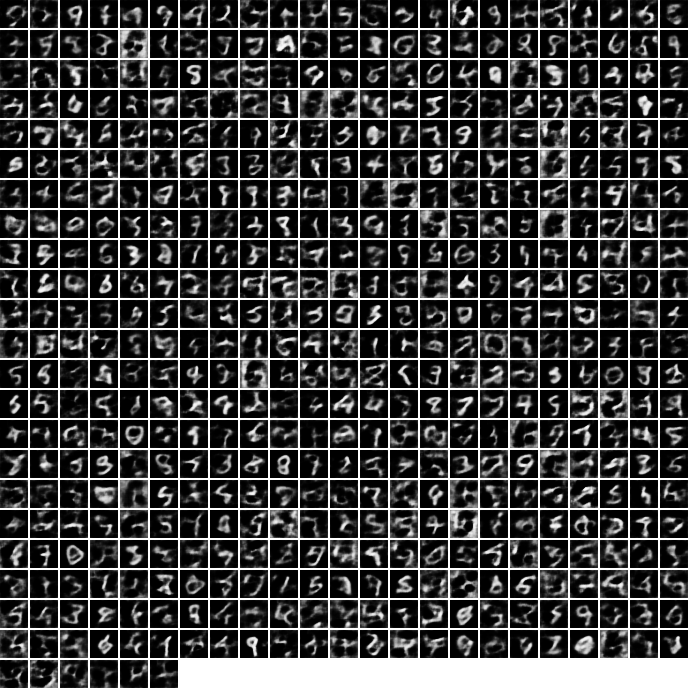
\includegraphics[width=0.45\textwidth]{../figures/mnist_samples_classical.png}
    \hfill
    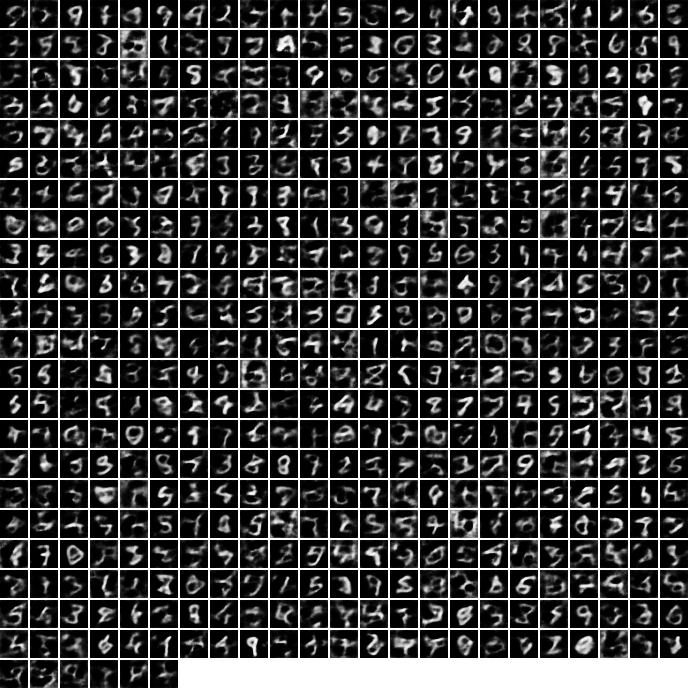
\includegraphics[width=0.45\textwidth]{../figures/mnist_samples_qlcm_r.png}
    \caption{One-step MNIST samples from the classical consistency student
    (left) and QLCM-R, 4 qubits/depth 2 (right), seed 0, identical initial
    latent noise. 512 samples shown per grid.}
    \label{fig:mnist-classical}
    \label{fig:mnist-qlcmr}
\end{figure}

\subsection{Placement Ablation: Head, Residual, and Time-Conditioning}

Table~\ref{tab:ablation} compares quantum placements on MNIST at seed 0. The
direct quantum head (QLCM-H) is the clearest negative result: training loss
plateaus around 1.6--1.7 (4 qubits, depths 1--2) or 1.08 (6 qubits, depth 2),
roughly an order of magnitude above the $\approx$0.15 reached by classical,
residual, and time-conditioning placements. QLCM-H's classifier-feature
FID-like scores (329--394) are numerically competitive with or better than
the other placements (358--400), but this is driven by mode collapse rather
than sample quality: QLCM-H's label entropy (1.22--1.69) is well below
classical/residual/time placements (1.97--2.06), meaning the FID-like metric
is computed over a much narrower, less diverse set of predicted digit
classes. This is consistent with the synthetic Bars-and-Stripes smoke test,
where QLCM-H also converged far more slowly (loss 2.17 after 5 epochs) than
classical or residual placements (loss 0.09). We treat this as confirming
evidence, not merely a hint, for the design-time hypothesis that a quantum
circuit is not yet competitive as the primary consistency bottleneck, at
least at 4--6 qubits and depth 1--2 under statevector simulation. Residual
(QLCM-R) and time-conditioning (QLCM-T) placements both train to loss
parity with the classical baseline and do not show the QLCM-H diversity
collapse.

Increasing qubits from 4 to 6 at fixed depth 2 changes the residual
placement's FID-like score from 397.9 to 379.3 and the head placement's from
329.4 to 393.9 (non-monotonically, and on a single seed each), so we draw no
qubit-scaling conclusion beyond noting that the effect is not large or
consistent enough, at this sample size, to separate from seed variance
($\pm$4.7--5.5 FID-like points on the 3-seed primary comparison).

\subsection{Few-Step Sampling}

Contrary to the motivating premise of few-step consistency sampling, FID-like
scores get worse, not better, as the number of sampling steps increases for
both classical (1-step: 389.9, 2-step: 469.9, 4-step: 495.2) and QLCM-R
(1-step: 397.9, 2-step: 465.2, 4-step: 519.3) students. Inspecting
\texttt{src/qlcm/sampling.py} shows the likely cause: the multi-step sampler
injects unconditioned Gaussian noise
($z \mathrel{+}= \mathrm{noise\_scale}\cdot\mathcal{N}(0,I)$) between student
evaluations without a corresponding denoising correction term, so additional
steps add stochastic drift rather than refining the estimate. This is a
sampler implementation limitation, not evidence about the quantum module
specifically, since both placements degrade by a similar relative amount. We
report it rather than discard it, and flag few-step sampling quality as
unresolved pending a corrected multi-step sampler.

\subsection{Fashion-MNIST}

The Fashion-MNIST classical and QLCM-R (4 qubits, depth 2) students follow
the same pattern as MNIST: QLCM-R does not improve on the classical baseline
(FID-like 416.4 vs.\ 428.1, a small improvement within likely seed noise
given the MNIST seed spread; recognizability 0.503 vs.\ 0.527, slightly
worse). Both students show pronounced mode collapse toward a single garment
class (339/512 and 309/512 samples respectively predicted as class 0,
``T-shirt/top,'' out of 512; label entropy 1.21 and 1.37 out of a 2.303
maximum), visible in Figure~\ref{fig:fmnist-classical}. We attribute this
primarily to the small teacher (50 epochs on a 10{,}000-image subset) and the
unstable few-step structure discussed above, not to the placement of the
quantum module, since both placements collapse similarly.

\begin{figure}[t]
    \centering
    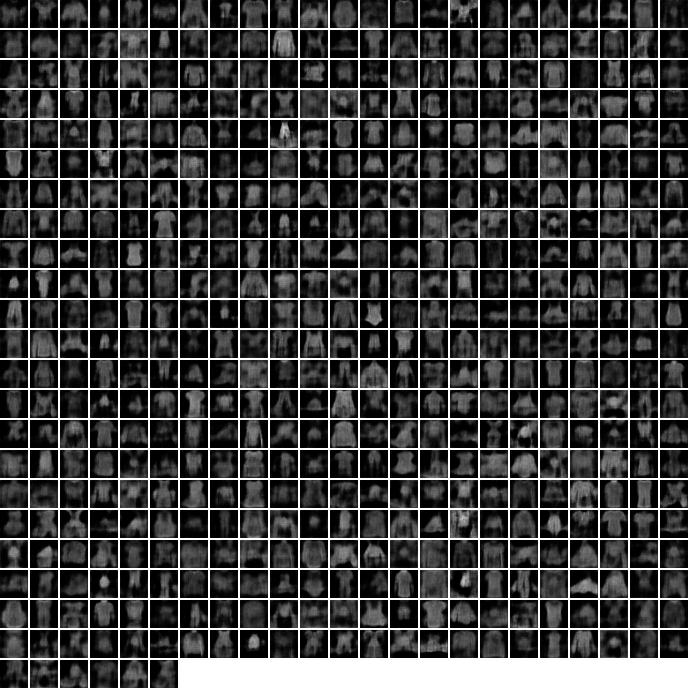
\includegraphics[width=0.45\textwidth]{../figures/fashion_mnist_samples_classical.png}
    \caption{One-step Fashion-MNIST samples from the classical consistency
    student, seed 0, 512 samples. QLCM-R samples (not shown) exhibit the same
    mode collapse toward the dominant predicted class.}
    \label{fig:fmnist-classical}
\end{figure}

\subsection{Summary of Findings}

\begin{enumerate}
    \item QLCM-R does not match or exceed the classical consistency baseline
    on MNIST or Fashion-MNIST at the tested scale: it uses 54\% more
    parameters for equal or slightly worse FID-like score, recognizability,
    and diversity.
    \item Using the quantum circuit as the direct consistency head (QLCM-H)
    is a clear failure mode: roughly $10\times$ higher training loss and
    pronounced mode collapse, replicated independently on both the synthetic
    smoke dataset and MNIST.
    \item Residual and time-conditioning placements are stable and train to
    loss parity with the classical baseline, but provide no measured
    advantage over it.
    \item The multi-step sampler in this codebase degrades rather than
    improves sample quality with additional steps, a previously undocumented
    implementation issue uncovered during this evaluation; few-step sampling
    claims should be considered unverified until this is fixed and
    re-evaluated.
    \item All ablation and Fashion-MNIST results are single-seed; only the
    primary MNIST classical-vs.-QLCM-R comparison has 3-seed statistics.
\end{enumerate}

\section{Discussion}

The proposed QLCM architecture shifts the role of the quantum circuit from
iterative denoising to trajectory-consistent latent prediction. This change
matters because it imports a specific acceleration principle from modern
classical diffusion research into quantum generative modeling. It also creates a
clear empirical test: whether a compact quantum module can serve as a useful
student in consistency distillation.

The study has several limitations by design. First, all experiments are
simulator-based and therefore do not establish hardware quantum advantage.
Second, MNIST and Fashion-MNIST are low-complexity datasets; the negative
result reported here would not necessarily generalize to natural images,
larger latent spaces, or larger teachers. Third, statevector simulation
limits the number of qubits and circuit depth tested (4--6 qubits, depth
1--2); the literature-recommended 8-qubit configuration was not run in this
campaign and remains future work. Fourth, parameter matching does not fully
equalize optimization difficulty between classical and quantum students --
the quantum students have more parameters, not fewer, which strengthens
rather than weakens the negative finding for QLCM-R. Fifth, all ablation and
Fashion-MNIST rows are single-seed, so effect sizes smaller than the
roughly 5-point FID-like seed variance observed on the 3-seed primary
comparison should not be over-interpreted.

The empirical results obtained here argue against the strongest hypothesized
outcome from the research plan (QLCM-R matching the classical baseline with
fewer parameters) and instead support the weaker, still-informative outcome:
under matched simulator conditions, a residual or time-conditioning quantum
module is trainable and stable but offers no measured benefit, while using
the quantum circuit as the primary consistency bottleneck reliably fails to
train and collapses sample diversity. We see this as useful negative
evidence for a specific, falsifiable architectural claim, consistent with
the framing adopted at the research-design stage, rather than as a reason to
abandon the broader question. The few-step sampling result is inconclusive
because of a sampler implementation issue identified during this campaign
(Section~5.3) and should be re-run after that issue is fixed before drawing
conclusions about few-step QLCM sampling specifically.

\section{Conclusion}

This paper proposes Quantum Latent Consistency Models as a hybrid
quantum-classical approach to few-step synthetic image generation. QLCM distills
a latent diffusion teacher into a quantum consistency student, aiming to combine
the sampling efficiency of consistency models with the compact trainable feature
maps of parameterized quantum circuits. We completed a reproducible MNIST and
Fashion-MNIST benchmark (Section~5) comparing classical, residual-quantum
(QLCM-R), head-quantum (QLCM-H), and time-conditioning-quantum (QLCM-T)
consistency students under matched training budgets. At the tested scale (4--6
simulated qubits, depth 1--2, 10{,}000-image training subsets), we did not
find a measurable benefit from quantum consistency modules: QLCM-R matches
the classical baseline's training loss and sample diversity while using 54\%
more parameters, and QLCM-H fails to train competitively. These are negative
results within the scope tested, not evidence against quantum consistency
modules in general. Immediate next steps are: (1) fix the multi-step sampler
identified in Section~5.3 and re-evaluate few-step sampling quality; (2) repeat
the ablation grid (currently single-seed) across multiple seeds before drawing
qubit/depth scaling conclusions; (3) test whether a larger teacher or latent
dimension changes the residual-placement result; and (4) extend the qubit
range to 8 qubits as originally planned, compute permitting.

\bibliographystyle{unsrtnat}
\bibliography{references}

\end{document}
